\documentclass{article}
\usepackage{amsmath}
\usepackage{amssymb}
\usepackage{geometry}
\usepackage{xcolor}
\usepackage{mdframed}
\geometry{a4paper, margin=1in, bottom=1cm}
\usepackage{multirow}
\usepackage{array}
\usepackage{booktabs}
\usepackage{tikz}
\usepackage{adjustbox}
\usepackage{graphicx}
\usepackage{parskip}
\usetikzlibrary{arrows,positioning}
\usepackage{caption}
\usepackage[spanish]{babel}

\title{Problemas de la Ruta más corta}
\author{Ricardo Largaespada}
\date{10 de marzo 2025}

\newmdenv[
  backgroundcolor=blue!5,
  linecolor=blue,
  linewidth=1pt,
  roundcorner=5pt,
  skipabove=\baselineskip,
  skipbelow=\baselineskip
]{problem}

\begin{document}

\maketitle

\begin{problem}\textbf{Ruta Más Confiable}

I. Q. Smart viaja diariamente en auto al trabajo. Sin embargo, la ruta más corta está altamente patrullada por la policía, lo que puede generar multas por exceso de velocidad. Para minimizar este riesgo, Smart ha decidido elegir la ruta que maximice la probabilidad de no ser detenido por la policía.

La red de posibles rutas se muestra en la Figura \ref{fig:reliable_path}, donde cada arco tiene asociada la probabilidad de no ser detenido en ese segmento. La probabilidad total de no ser multado en una ruta es el producto de las probabilidades de sus segmentos. 

El problema puede reformularse como un modelo de ruta más corta utilizando una transformación logarítmica para convertir el producto de probabilidades en una suma de logaritmos. Es decir, para una ruta \( p_{1k} = p_1 \times p_2 \times \dots \times p_k \), aplicamos logaritmos para obtener:

\[
\log p_{1k} = \log p_1 + \log p_2 + \dots + \log p_k
\]

Dado que la función logarítmica es monótona creciente, maximizar \( p_{1k} \) equivale a minimizar \( -\log p_{1k} \). Así, el problema se convierte en encontrar la ruta más corta en una nueva red donde los valores de los arcos son \( -\log p_{ij} \).

\begin{center}
    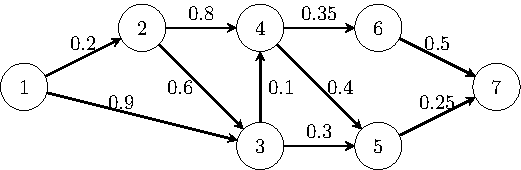
\includegraphics[scale=1]{images/reliable_path.pdf}
    \captionof{figure}{Modelo de red para la ruta más confiable.}
    \label{fig:reliable_path}
\end{center}


\textbf{Tarea:} Aplicar el algoritmo de Dijkstra en la red transformada para encontrar la ruta más confiable desde el nodo de origen hasta el destino.
\end{problem}

\begin{problem}
\textbf{Enrutamiento de Mensajes en una Red de Telecomunicaciones}

La empresa de telefonía celular \textit{Tell-All} brinda servicio a seis áreas geográficas conectadas por enlaces satelitales. Las distancias entre estas áreas se muestran en la Figura \ref{fig:telecom_network}, con valores en millas.

\textbf{Objetivo:} Determinar las rutas más eficientes para enviar mensajes entre cada par de áreas, minimizando la distancia total.

\textbf{Tarea:}  
\begin{enumerate}
    \item Aplicar el algoritmo de Dijkstra desde el nodo 1 para encontrar la ruta más corta a los demás nodos.
\end{enumerate}

\begin{center}
\begin{tikzpicture}[scale=1, transform shape]

    % Definir nodos con posiciones específicas
    \node[circle, draw, minimum size=0.8cm] (n1) at (0,1) {1};
    \node[circle, draw, minimum size=0.8cm] (n2) at (2,3) {2};
    \node[circle, draw, minimum size=0.8cm] (n3) at (2,0) {3};
    \node[circle, draw, minimum size=0.8cm] (n4) at (4,1.5) {4};
    \node[circle, draw, minimum size=0.8cm] (n5) at (6,0) {5};
    \node[circle, draw, minimum size=0.8cm] (n6) at (6,3) {6};

    % Definir aristas con pesos
    \path[draw, thick]
    (n1) edge node[left] {700} (n2)
    (n1) edge node[left] {200} (n3)
    (n2) edge node[left] {300} (n3)
    (n2) edge node[above] {400} (n6)
    (n2) edge node[above] {200} (n4)
    (n3) edge node[below] {700} (n4)
    (n3) edge node[below] {600} (n5)
    (n4) edge node[above] {100} (n6)
    (n4) edge node[below] {300} (n5)
    (n5) edge node[right] {500} (n6);

\end{tikzpicture}
\end{center}
\captionof{figure}{Red de telecomunicaciones de Tell-All.}
\label{fig:telecom_network}
\end{problem}

\begin{problem}
\textbf{Optimización de Rutas en un Sistema de Transporte}

Se tiene un sistema de transporte modelado mediante la red de la Figura \ref{fig:transport_network}. Cada nodo representa un punto de la ciudad y cada arista indica la distancia entre ellos. Se necesita encontrar la mejor ruta desde un punto de origen hasta un destino, minimizando la distancia total recorrida.

\textbf{Tarea:}  
\begin{enumerate}
    \item Aplicar el algoritmo de Floyd-Warshall para obtener la matriz de distancias mínimas entre todos los nodos.
\end{enumerate}

\begin{center}
    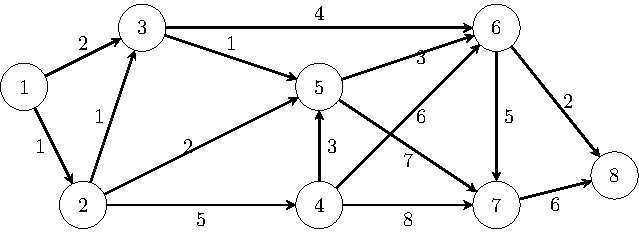
\includegraphics[width=0.7\textwidth]{images/transport_network.pdf}
\end{center}
\captionof{figure}{Red del sistema de transporte.}
\label{fig:transport_network}
\end{problem}

\end{document}
